\chapter{A \ReplicaGenOne{} beállítása és karbantartása}\label{ch:replica-setup}

Ez a fejezet a klasszikus \ReplicaGenOne{} műszeregységre vonatkozik, amelyet a \autoref{fig:replica-classic} ábra mutat. Ha a műszer a \ReplicaNextLong{} elrendezését követi, használja az előző fejezetet.

\begin{figure}[htbp]
    \centering
    \begin{subfigure}{0.46\textwidth}
        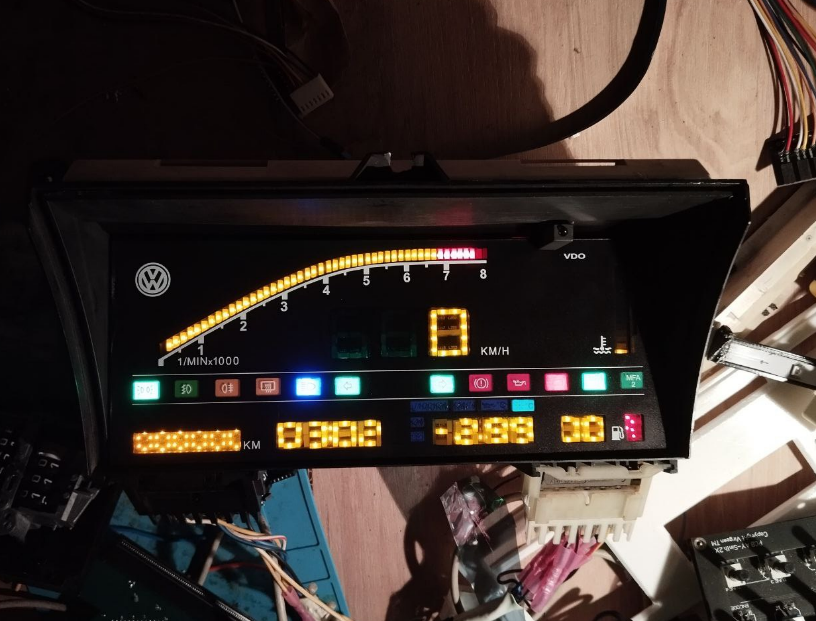
\includegraphics[width=\linewidth]{digifiz_manual/image046.png}
        \caption{Klasszikus \ReplicaGenOne{} szögletes kerettel.}
    \end{subfigure}\hfill
    \begin{subfigure}{0.46\textwidth}
        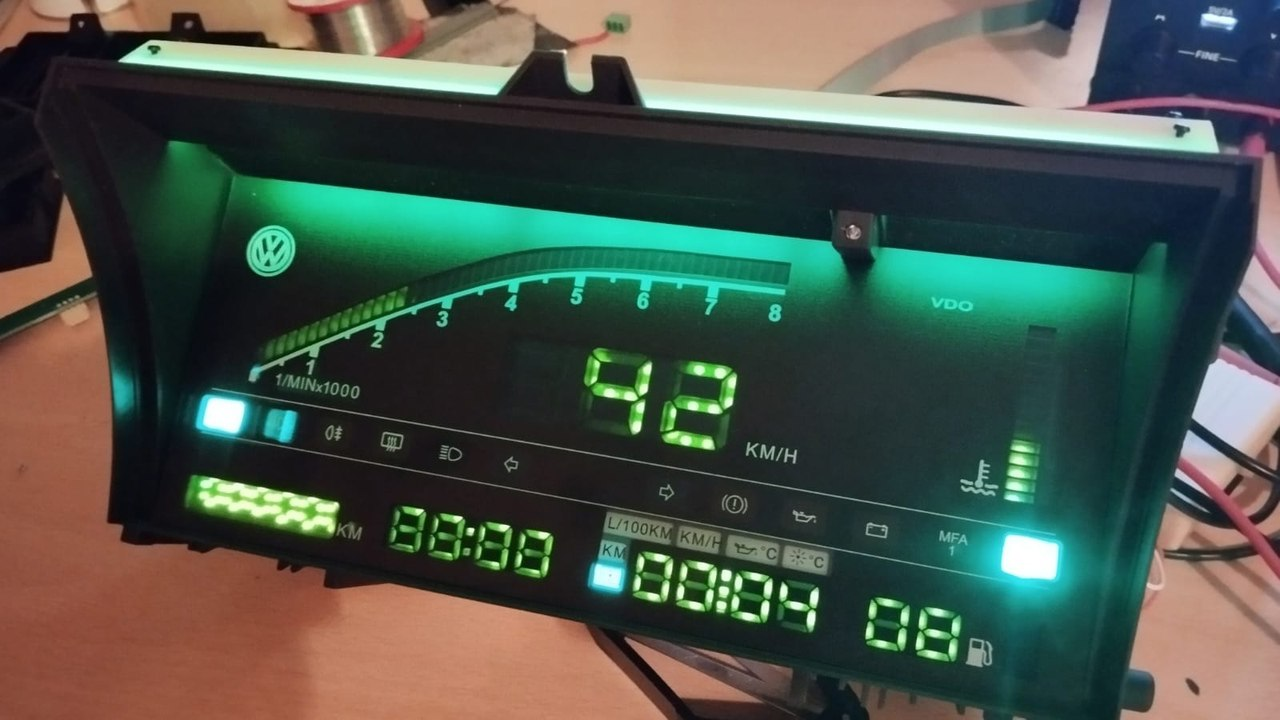
\includegraphics[width=\linewidth]{digifiz_manual/image047.png}
        \caption{Lekerekített előlap a későbbi készleteken.}
    \end{subfigure}
    \caption{A \ReplicaGenOne{} műszerfal megjelenése.}
    \label{fig:replica-classic}
\end{figure}

\section{Kezelés és kijelzőápolás}
\begin{itemize}
    \item Az UV-nyomtatott plexi előlap könnyen karcolódik. Kerülje az éles vagy csiszoló anyagokkal való érintkezést.
    \item A felületi sérülés esztétikai jellegű, és nem garanciális. Deformált minta esetén rendeljen cserealkatrészt a PHOL-LABS Kft.-től.
\end{itemize}

\section{Valós idejű óra eleme}
A műszerben DS3231 valós idejű óra dolgozik CR2032 gombelemmel. Az elem jellemzően körülbelül négy évig tart; lemerüléskor az óra minden bekapcsolásnál alaphelyzetbe áll. A front- és/vagy hátlap eltávolítása után, a kábelezés leválasztása nélkül cserélje ki a cellát. A használt elemet a helyi szabályozás szerint selejtezze.

\section{Firmware karbantartása USBasp programozóval}
Minden készlethez USBasp programozókábelt mellékelünk, amelyet előre bekötve talál a házban (\autoref{fig:usbasp-cable}). A villogtatás előtt telepítsen megfelelő USBasp illesztőprogramot, például a következő címről:
\displayurl{https://myrobot.ru/downloads/driver-usbasp-v-2.0-usb-isp-windows-7-8-10-xp.php}
A programozó a számítógéphez csatlakoztatva tápot ad a műszernek, így padon is ellenőrizhető.

\begin{figure}[htbp]
    \centering
    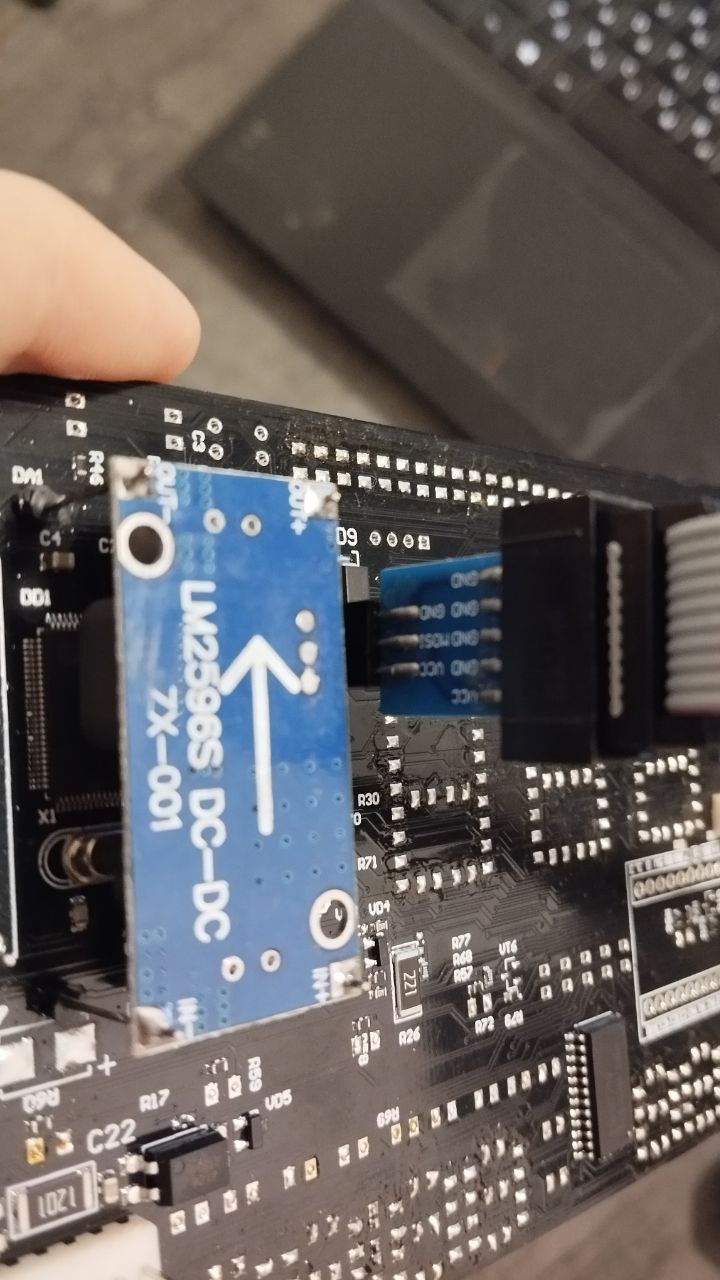
\includegraphics[width=0.32\textwidth]{digifiz_manual/image048.png}
    \caption{Az USBasp kábel tájolása a \ReplicaGenOne{} belsejében.}
    \label{fig:usbasp-cable}
\end{figure}

A firmware-t \texttt{avrdude} segédprogrammal villogtassa az alábbi paranccsal (szükség esetén módosítsa a fájlnevet):

\begin{verbatim}
avrdude -c usbasp -p m2560 -e \
    -U lfuse:w:0xff:m -U hfuse:w:0x99:m -U efuse:w:0xff:m \
    -U flash:w:Digifiz.ino.mega.hex
\end{verbatim}

Sikeres feltöltés után nyomja meg a frontoldali érintőgombot négyszer-ötször a memória blokkok inicializálásához. Ha a blokkok üresek maradnak, ismételje meg a villogtatást, vagy küldje el a Bluetooth \verb|252 0| parancsot a gyári visszaállításhoz. A kész firmware képfájlok itt érhetők el:
\displayurl{https://github.com/Sgw32/DigifizReplica}

\section{Bluetooth konfiguráció}
A legtöbb paraméter Bluetoothon, Android telefon és Serial Bluetooth Terminal alkalmazás segítségével állítható. Párosítás előtt töltse le az alábbi hivatkozásról:
\displayurl{https://play.google.com/store/apps/details?id=de.kai_morich.serial_bluetooth_terminal&hl=en&gl=US}
iOS eszközök nem tudnak csatlakozni a klasszikus Bluetooth 2.0 modulhoz.

\begin{itemize}
    \item Győződjön meg róla, hogy a műszer Bluetooth Classic interfészével párosít, ne csak BLE eszközökkel.
    \item A Serial Bluetooth Terminalban állítsa a sorvégjelet LF-re, és kapcsolja ki a CR+LF módot parancsok küldése előtt.
\end{itemize}

\begin{figure}[htbp]
    \centering
    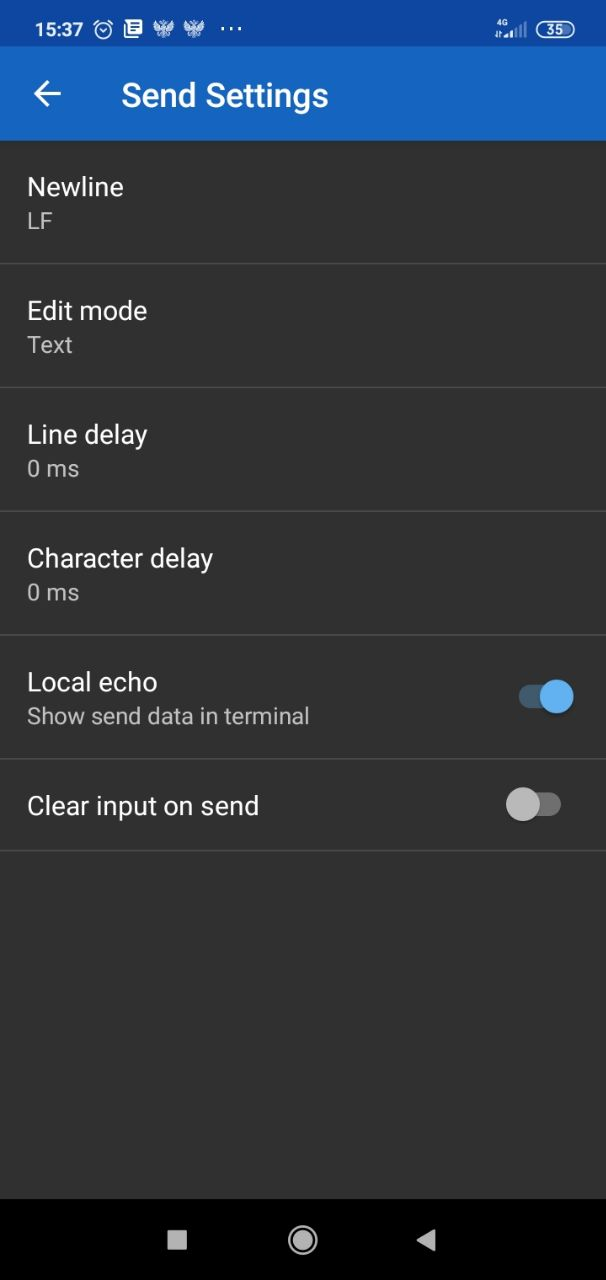
\includegraphics[width=0.32\textwidth]{digifiz_manual/image049.png}
    \caption{Ajánlott Serial Bluetooth Terminal beállítások.}
    \label{fig:sbt-settings}
\end{figure}

A parancsokat szóközzel elválasztott \verb|<szám> <érték>| párokként adja meg. Például a 123\,456~km futásteljesítmény tárolásához küldje el a \verb|11 123456| parancsot. Egy parancs aktuális értékének lekérdezéséhez adjon hozzá 128-at a számához (a \verb|129 0| visszaadja a sebességkorrekciós tényezőt). A \verb|adc 0| diagnosztikai parancs nyers szenzoradatokat jelenít meg, amelyek segítenek a hibák feltárásában.

\section{Konfigurációs paraméterek}
A legfontosabb Bluetooth parancsokat a \autoref{tbl:replica-classic-commands} táblázat sorolja fel. Az 1/1.5 és 2. generációs műszerek alapbeállításait a \autoref{tbl:replica-defaults} összegzi. A 31--33 parancsokat csak \ReplicaNextShort{} egységeken használja; a klasszikus \ReplicaGenOneShort{} esetén nincs hatásuk.

{\scriptsize
\begin{longtblr}[
    caption = {Klasszikus \ReplicaGenOne{} konfigurációs parancsok.},
    label = {tbl:replica-classic-commands},
]{
    colspec = {Q[c,0.14\linewidth] >{\ttfamily}Q[l,0.38\linewidth] Q[l]},
    rowsep = 2pt,
}
    \toprule
    \textbf{Azonosító} & \textbf{Név} & \textbf{Leírás} \\
    \midrule
    22 (vagy 0) & PARAMETER\_RPMCOEFFICIENT & Motorfordulatszám-korrekciós tényező. \\
    1 & PARAMETER\_SPEEDCOEFFICIENT & Sebességkorrekciós tényező. \\
    2 & PARAMETER\_COOLANTTHERMISTORB & Hűtőfolyadék termisztor béta tényező. \\
    3 & PARAMETER\_OILTHERMISTORB & Olaj termisztor béta tényező. \\
    4 & PARAMETER\_AIRTHERMISTORB & Külső levegő termisztor béta tényező. \\
    5 & PARAMETER\_TANKMINRESISTANCE & Minimális üzemanyagszint-ellenállás (\si{\ohm}). \\
    6 & PARAMETER\_TANKMAXRESISTANCE & Maximális üzemanyagszint-ellenállás (\si{\ohm}). \\
    7 & PARAMETER\_TAU\_COOLANT & Hűtőfolyadék hőmérséklet szűrőállandó. \\
    8 & PARAMETER\_TAU\_OIL & Olajhőmérséklet szűrőállandó. \\
    9 & PARAMETER\_TAU\_AIR & Külső hőmérséklet szűrőállandó. \\
    10 & PARAMETER\_TAU\_TANK & Üzemanyagszint szűrőállandó. \\
    11 & PARAMETER\_MILEAGE & Összesített kilométer-számláló. \\
    12 & PARAMETER\_DAILY\_MILEAGE & Napi számláló. \\
    13 & PARAMETER\_AUTO\_BRIGHTNESS & Automatikus fényerő engedélyezése. \\
    14 & PARAMETER\_BRIGHTNESS\_LEVEL & Kézi fényerő szint (0--15). \\
    15 & PARAMETER\_TANK\_CAPACITY & Üzemanyagtartály kapacitása (liter). \\
    16 & PARAMETER\_MFA\_STATE & Aktív MFA oldal. \\
    17 & PARAMETER\_BUZZER\_OFF & Hangjelző letiltása (1 tilt, 0 engedélyez). \\
    18 & PARAMETER\_MAX\_RPM & Fordulatszámmérő skála (alap 8000). \\
    19 & PARAMETER\_NORMAL\_RESISTANCE\_COOLANT & Hűtő jeladó ellenállása \SI{25}{\celsius}-on. \\
    20 & PARAMETER\_NORMAL\_RESISTANCE\_OIL & Olaj jeladó ellenállása \SI{25}{\celsius}-on. \\
    21 & PARAMETER\_NORMAL\_RESISTANCE\_AMB & Külső jeladó ellenállása \SI{25}{\celsius}-on. \\
    23 & PARAMETER\_DOT\_OFF & Óra kettőspont viselkedése (0 villog, 1 folyamatos). \\
    24 & PARAMETER\_BACKLIGHT\_ON & Háttérvilágítás bekapcsolása tompított fénnyel. \\
    25 & PARAMETER\_M\_D\_FILTER & Mediánszűrő állandó (örökölt). \\
    26 & PARAMETER\_COOLANT\_MAX\_R & Hűtő „teljes skálás” hőmérséklet küszöb. \\
    27 & PARAMETER\_COOLANT\_MIN\_R & Hűtő „1~bar” hőmérséklet küszöb. \\
    31--33 & PARAMETER\_MAINCOLOR\_[RGB] & Felhasználói felület színei (csak \ReplicaNextShort{}). \\
    37 & PARAMETER\_RPM\_FILTER & Fordulatszám-szűrő agresszivitás. \\
    128 & PARAMETER\_READ\_ADDITION & Hozzáadandó érték paraméter olvasáshoz. \\
    255 & PARAMETER\_SET\_HOUR & Óra beállítása (24 órás). \\
    254 & PARAMETER\_SET\_MINUTE & Perc beállítása. \\
    253 & PARAMETER\_RESET\_DAILY\_MILEAGE & Napi számláló nullázása. \\
    252 & PARAMETER\_RESET\_DIGITAL & Gyári visszaállítás és memória inicializálás. \\
    \bottomrule
\end{longtblr}}

A Serial Bluetooth Terminal gyorsgombjai hasznosak a rutinfeladatokhoz, például az automatikus fényerő ki- és bekapcsolásához (\verb|13 0|, \verb|13 1|) vagy a színértékek írásához. 60~\%-nál magasabb fényerőt csak rövid tesztekhez használjon, hogy megőrizze a LED-ek élettartamát.
